% This file is part of the stream_information project.
% Copyright 2017 the authors. All rights reserved.

% # style notes
% - it is Cram\'er--Rao not Cram\'er-Rao. And yet Fisher-matrix not Fisher--matrix.

% TODO:
% - Reference for the dustmaps package? See software section.

\documentclass[modern]{aastex62}

\usepackage{amsmath}

% typography
\setlength{\parindent}{1.\baselineskip}
\newcommand{\acronym}[1]{{\small{#1}}}
\newcommand{\package}[1]{\textsl{#1}}
\newcommand{\gaia}{\textsl{Gaia}}
\newcommand{\DR}{\acronym{DR2}}

% aastex parameters
% \received{not yet; THIS IS A DRAFT}
%\revised{not yet}
%\accepted{not yet}
% % Adds "Submitted to " the arguement.
% \submitjournal{ApJ}
\shorttitle{GD-1 in Gaia DR2}
\shortauthors{price-whelan \& bonaca}

%@arxiver{}

\begin{document}\sloppy\sloppypar\raggedbottom\frenchspacing % trust me

\title{Gaia DR2 view of the GD-1 stellar stream}

\author[0000-0003-0872-7098]{Adrian~M.~Price-Whelan}
\affiliation{Department of Astrophysical Sciences,
             Princeton University, Princeton, NJ 08544, USA}
\email{adrn@astro.princeton.edu}
\correspondingauthor{Adrian M. Price-Whelan}

\author[0000-0002-7846-9787]{Ana Bonaca}
\affil{Harvard--Smithsonian Center for Astrophysics, Cambridge, MA 02138, USA}


\begin{abstract}\noindent % trust me
Tidally-disrupted globular clusters leave behind thin, dynamically-cold streams
of stars that are extremely valuable tracers of the large- and small-scale
properties of mass around the Galaxy.
Many thin stellar streams have been discovered around the Milky Way, the
majority of which exist in the Galactic halo and are therefore primarily
sensitive to the distribution of dark matter.
Here we present astrometric data for one of the longest stellar streams --- the
``GD-1'' stream --- from data release 2 (\DR) of the \gaia\ mission.
We re-discover significant density variations along the stream by selecting
candidate member stars using the exquisite \gaia\ data alone.
Combined with filtering using Pan-STARRS photometry, we see clear evidence of a
prominent, apparent gap in the stream, and at least XX other under-densities.
These density variations --- and especially the gap --- are possible indications
of past interactions with large, massive perturbers such as dark matter
sub-halos.
\end{abstract}

\keywords{Galaxy: halo --- dark matter}

\section{Introduction}
\label{sec:intro}

Dynamically cold stellar streams, likely formed from the tidal disruption of globular clusters, are sensitive to the large and small scale distribution of matter in the halo

Thin stellar streams form from the tidal disruption of low-dispersion stellar systems such as globular clusters \citep[e.g.,][]{TODO}. To date, $\approx$13--14 thin streams have been discovered by searching large-area sky surveys such as the Sloan Digital Sky Survey (SDSS) and Pan-STARRS1 survey (PS1). These previously known thin streams span a wide range of lengths \citep[$\sim$$2$--$60$ deg;][]{bernard14,grillmair06} and masses \citep[$\sim$$10^3$--$10^5~\msun$;][]{TODO,TODO}, however, only two such streams have clear progenitor systems: NGC 5466 and Palomar 5 \citep{TODO,TODO}. Though it has been shown with many independent methods that modeling these thin streams can place strong constraints on the gravitational potential in which they form \citep{apw14,TODO}, many efforts to apply these models to real streams around the Milky Way have been hampered by the small number of known progenitor systems.


\section{Data}
\label{sec:data}


Most of the clearly identifiable portions of the GD-1 stream are located at high
Galactic latitudes ($b > 35^\circ$), and we therefore do not expect significant
dust extinction or variations in extinction along the stream.
\figurename~\ref{fig:sfd} shows the $V$-band extinction in the region around the
GD-1 stream, computed from the Schlegel-Finkbeiner-Davis extinction map
(\cite{Schlegel:1998}; hereafter SFD).
Vertical lines indicate the two regions clearly identifiable as under-densities
from the proper-motion-selected stream members.
The maximum $A_V$ is $\approx$0.07 mag in both the under-density and gap
regions.
The dispersion in $A_V$ in the region $-60^\circ < \phi_1 < 0^\circ$ and
$-1^\circ < \phi_1 < 1^\circ$ is $\std_{A_V} \approx 0.03~\textrm{mag}$.

% Notebook: GD1-dust-and-completeness
\begin{figure}[h]
\begin{center}
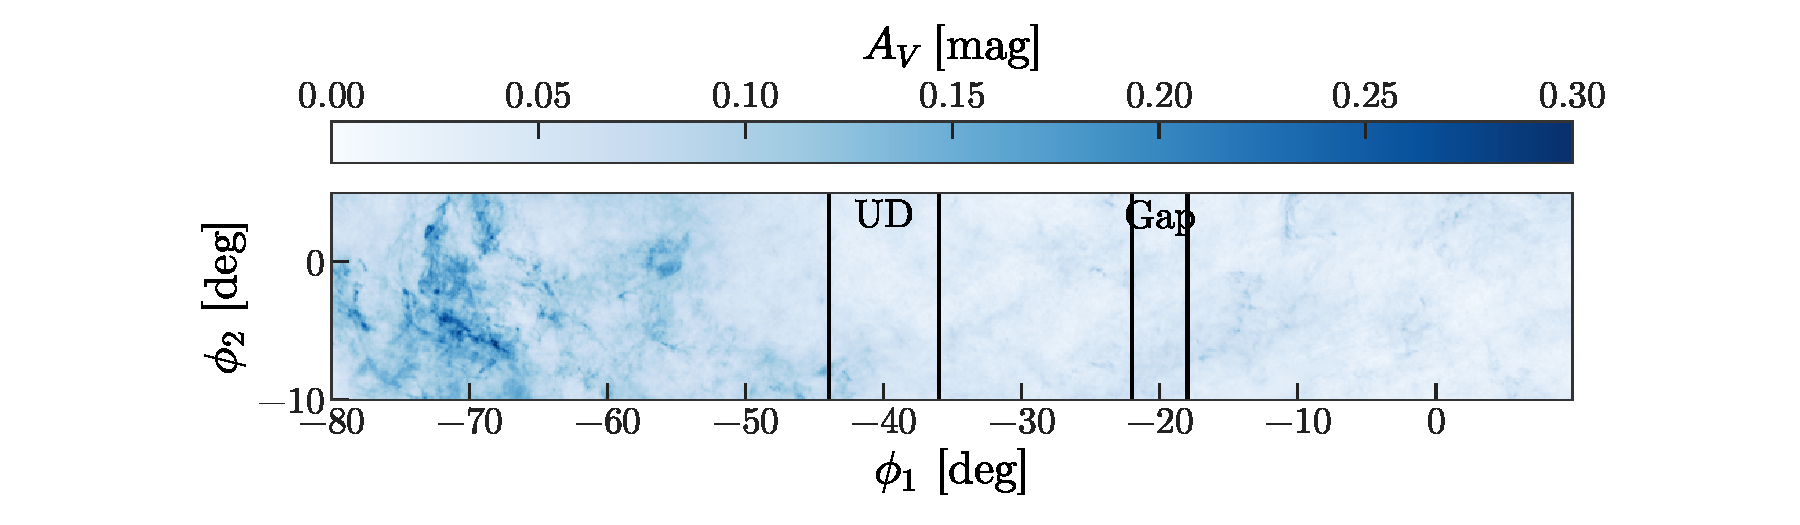
\includegraphics[width=\textwidth]{sfd.pdf}
\end{center}
\caption{%
Colored background shows the \gaia\ $G$-band extinction, $A_G$, in the GD-1
coordinate system.
Vertical lines roughly show the regions identified as the under-density (UD) and
gap.
The maximum extinction in the UD or Gap regions is $\approx$0.07 mag.
\label{fig:sfd}
}
\end{figure}


\section{Results}
\label{sec:results}

\subsection{Global properties}
\label{sec:res_global}

\subsection{Gap}
\label{sec:res_gap}

\subsection{Underdensity}
\label{sec:res_underdensity}


\section{Discussion}
\label{sec:discussion}


\acknowledgements{
thanks: Belokurov, Casey, Geha, Hogg, Johnston, Koposov, Schlafly, Spergel
This research was started at the NYC Gaia DR2 Workshop at the Center for Computational Astrophysics of the Flatiron Institute in 2018 April.
AB acknowledges generous support from the Institute for Theory and Computation at Harvard University.
All code used in this work and all results are available at \url{https://github.com/adrn/GD1-DR2}.
}

\software{
    \package{Astropy} \citep{astropy},
    \package{dustmaps}\footnote{\url{https://github.com/gregreen/dustmaps}},
    \package{gala} \citep{gala},
    \package{IPython} \citep{ipython},
    \package{matplotlib} \citep{mpl},
    \package{numpy} \citep{numpy},
    \package{scipy} \citep{scipy}
}

\bibliographystyle{aasjournal}
\bibliography{gd1}

\clearpage

\appendix
\section{Completeness check and data validation}
\label{sec:validate}

% % Notebook:
% \begin{figure}[h]
% \begin{center}
% \includegraphics[width=0.7\textwidth]{nvisits.pdf}
% \end{center}
% \caption{%
% TODO
% \label{fig:TODO}
% }
% \end{figure}


\end{document}
